\documentclass[11pt,a4paper]{article}

% ---------- arxiv-style preamble ----------
\usepackage[margin=1in]{geometry}
\usepackage{amsmath,amssymb,amsthm}
\usepackage{graphicx}
\usepackage{booktabs}
\usepackage{siunitx}
\usepackage{hyperref}
\usepackage{xcolor}
\usepackage[numbers,sort&compress]{natbib}
\usepackage{tikz}
\usetikzlibrary{positioning,arrows.meta}
\usepackage{pgfplots}
\pgfplotsset{compat=1.18}
\usepackage{caption}
\usepackage{listings}
\usepackage{array}
\captionsetup{font=small,labelfont=bf}
\hypersetup{
  colorlinks=true,
  linkcolor=blue!50!black,
  citecolor=blue!50!black,
  urlcolor=blue!50!black
}

\providecommand{\tierBlue}{🔵}
\providecommand{\tierGreen}{🟢}
\providecommand{\tierYellow}{🟡}
\providecommand{\tierOrange}{🟠}
\providecommand{\tierRed}{🔴}

\newtheorem{theorem}{Theorem}

\title{
  \textbf{RTSC Ambient Roadmap}\\[4pt]
  \large An $m$-Margin Unification of Allen--Dynes Closed-Form and Anharmonic Stability,
  with YH$_{10}$ as the First Measured ESCAPE-Class Candidate
}

\author{
  \texttt{hexa-lang} maintainers\\
  \normalsize\textit{dancinlab}\\[2pt]
  \normalsize\href{https://github.com/dancinlab/hexa-lang}{\texttt{github.com/dancinlab/hexa-lang}}
}

\date{\today}

\begin{document}

\maketitle

% =========================================================================
\begin{abstract}
We close the math DFS lane of the room-temperature superconductor (RTSC)
problem with eighteen rounds of inline closed-form verification, totalling
seventy verify-points (forty-nine \tierGreen\ SUPPORTED-NUMERICAL,
four \tierRed\ FALSIFIED honest closed-negatives, zero \tierOrange/\tierYellow/\textcircled{w}).
The key contribution is an $m$-margin grand unification: the Allen--Dynes
closed-form $293$\,K iso-line and the anharmonic stability
\texttt{stability\_coupling\_margin} are shown to be \emph{two
representations of the same single function}, with the sign of
$m=(\langle\omega^2\rangle_{\text{anharm}}-\langle\omega^2\rangle_\lambda)/
\langle\omega^2\rangle_{\text{anharm}}$ deciding whether a hydride family is
TRAPPED (binary, $m<0$) or ESCAPE-able (clathrate-ternary, $m>0$). Applied
to the literature parameter tuples for H$_3$S, LaH$_{10}$, YH$_{10}$ and
CaH$_6$, the classification reveals YH$_{10}$ at $m=+0.035$ as the first
measured candidate already inside the ESCAPE region (Errea \emph{et~al.}
2020), alongside the Wang--Ma 2012 CaH$_6$ anchor at $m=+0.074$. The
$293$\,K closed-form prediction is: LaH$_{10}$-class ternaries require a
$+18\%$ enhancement of $\lambda$ (achievable by ternary doping), whereas
binary H$_3$S would need $+50\%$ which is unphysical at ambient pressure.
We close the lane with an honest model tension: the standard
$\mu_{\text{bare}}=0.3$ Morel--Anderson assumption is $+33{-}70\%$ over the
fit-back $\mu^*$ from measured $T_c$, so the real $\mu_{\text{bare}}$ is
$0.14{-}0.20$ (high-pressure hydride strong $e$-ph screening). Verification
data persists in \texttt{companion/verify-ledger.json}; every closed-form
in the paper is an inline \texttt{hexa verify --expr} call with the
verbatim verdict.
\end{abstract}

\section{Introduction}
\label{sec:intro}

The room-temperature superconductor (RTSC) target of $293$\,K at ambient
pressure has been the focus of high-pressure hydride research since the
H$_3$S discovery of Drozdov \emph{et~al.}~\cite{drozdov2015}. The subsequent
LaH$_{10}$ measurement at $250$\,K under $170$\,GPa~\cite{somayazulu2019}
and the theoretical prediction of YH$_{10}$ at $303$\,K under $250$\,GPa
by Errea \emph{et~al.}~\cite{errea2020} have driven the field toward
clathrate-class ternaries, while the binary class appears stalled below
$220$\,K. The mechanistic root of this binary--ternary divide has been
the subject of two parallel literatures: (i) the Allen--Dynes
closed-form analysis of phonon-mediated $T_c$~\cite{allenDynes1975}, and
(ii) the anharmonic-stability budget tracked through the Hopfield
parameter~\cite{hopfield1969} and the SSCHA-corrected phonon
spectrum~\cite{errea2014sscha}. These have been treated as complementary
but distinct.

In this paper we show that, in fact, the two literatures are
\emph{two representations of the same single closed-form function} ---
the stability-coupling margin $m$ --- and that the
sign of $m$ is the binary/ternary discriminant.

\medskip
\noindent\textbf{Contributions.}
\begin{enumerate}\itemsep0.3em
\item \textbf{$m$-margin grand unification.} The Allen--Dynes
$293$\,K iso-line (Section~\ref{sec:results-iso}) and the anharmonic
stability margin (Section~\ref{sec:results-margin}) are the same single
closed-form function viewed with two normalisations (Theorem~\ref{thm:unify}).
\item \textbf{YH$_{10}$ as first measured ESCAPE candidate.} Applying the
unified $m$-margin to the literature parameter tuples for four hydrides
yields a sign classification (Table~\ref{tab:m-classification}) in which
YH$_{10}$ at $m=+0.035$ joins CaH$_6$ at $m=+0.074$ as the only
measured/predicted candidates already in the ESCAPE region.
\item \textbf{Honest model tension.} The standard
$\mu_{\text{bare}}=0.3$ Morel--Anderson assumption~\cite{morelAnderson1962}
disagrees with the fit-back $\mu^*$ from measured $T_c$ by $+33$ to
$+70\%$ across H$_3$S and LaH$_{10}$, implying a system-dependent
$\mu_{\text{bare}}\in[0.14,0.20]$ for high-pressure hydrides. We do
not paper over this tension; it is registered as a \tierRed\ closed
negative against the canonical $\mu_{\text{bare}}=0.3$ literature
default (Section~\ref{sec:limits}).
\end{enumerate}

\section{Background}
\label{sec:bg}

The phonon-mediated $T_c$ closed-form of Allen--Dynes~\cite{allenDynes1975},
in its simple-AD form, reads
\begin{equation}
\label{eq:adsimple}
T_c^{\text{simple-AD}} = \frac{\omega_{\log}}{1.2}\,
\exp\!\Bigl[-\frac{1.04(1+\lambda)}{\lambda-\mu^*(1+0.62\lambda)}\Bigr],
\end{equation}
where $\lambda$ is the McMillan coupling, $\omega_{\log}$ the logarithmic
average phonon frequency, and $\mu^*$ the Coulomb pseudopotential. The
full-AD form adds the strong-coupling correction factor
$f_1\!\cdot\!f_2$ \cite{allenDynes1975}. The Morel--Anderson Tolmachev
log renormalisation~\cite{morelAnderson1962} relates the bare and screened
Coulomb couplings,
\begin{equation}
\label{eq:ma}
\mu^* = \frac{\mu_{\text{bare}}}{1+\mu_{\text{bare}}\ln(E_F/\omega_{\text{ph}})}.
\end{equation}

The anharmonic-stability margin of Hopfield~\cite{hopfield1969} with
SSCHA correction~\cite{errea2014sscha} introduces a stiffness
$\langle\omega^2\rangle_{\text{anharm}}$ and a coupling-required stiffness
$\langle\omega^2\rangle_\lambda=\eta/(M\lambda_{\text{target}})$ where
$\eta$ is the Hopfield electronic factor and $M$ the cation mass. The
margin reads
\begin{equation}
\label{eq:margin}
m = \frac{\langle\omega^2\rangle_{\text{anharm}}-\langle\omega^2\rangle_\lambda}
       {\langle\omega^2\rangle_{\text{anharm}}}.
\end{equation}
The Wang--Ma~2012 CaH$_6$ cation pre-compression anchor~\cite{wangMa2012}
gives the canonical anchor $m=+0.5$ (\(\langle\omega^2\rangle_{\text{anharm}}=1.0\),
\(\langle\omega^2\rangle_\lambda=0.5\)); the binary h$_3$o anchor gives
$m=-1.479$.

\medskip
\noindent The Eliashberg framework~\cite{carbotte1990} extends BCS by
keeping the retarded structure of the phonon-mediated interaction
through the spectral function $\alpha^2 F(\omega)$. The coupling enters
through the ω⁻¹-weighted moment
$M_0 = \int_0^\infty \alpha^2 F(\omega)/\omega\,d\omega$ with
$\lambda = 2 M_0$, and the logarithmic average phonon frequency
$\omega_{\log}$ is the second moment that selects the relevant phonon
energy scale~\cite{allenDynes1975}. The Allen--Dynes closed-form
of Eq.~\ref{eq:adsimple} is the asymptotic ``best fit'' to the full
Eliashberg solution in the strong-coupling regime $\lambda\in[1,2]$,
with the $f_1\!\cdot\!f_2$ correction extending it to $\lambda\sim 3$.
Above $\lambda\sim 5$ the Allen--Dynes form diverges and direct
Eliashberg numerical integration is required~\cite{carbotte1990}.
The math DFS lane of this paper deliberately stays inside the
$\lambda\in[1.3, 3.5]$ envelope where Allen--Dynes is closed-form
trustworthy; the deferred Eliashberg numerical solver
(Section~\ref{sec:limits}, item 3) is the natural extension when the
closed-form regime is exhausted.

\medskip
\noindent The chronological context of the field is short. Drozdov
\emph{et~al.}~2015~\cite{drozdov2015} reported $T_c=203$\,K in H$_3$S
at $155$\,GPa, the first sub-room-temperature conventional
superconductor. Somayazulu \emph{et~al.}~2019~\cite{somayazulu2019}
measured LaH$_{10}$ at $T_c=250$\,K and $170$\,GPa, with the
clathrate-class quantum-crystal structure subsequently confirmed by
Errea \emph{et~al.}~2020~\cite{errea2020} via SSCHA. The same Errea
team predicted YH$_{10}$ at $T_c=303$\,K and $250$\,GPa
(literature $\lambda=2.59$, $\omega_{\log}\approx 1500$\,K). The
canonical anchor on the anharmonic-stability side is the CaH$_6$
sodalite-like clathrate prediction of Wang--Ma~2012~\cite{wangMa2012}
which introduced the cation pre-compression mechanism that makes
$\langle\omega^2\rangle_{\text{anharm}}$ large enough to push $m>0$.

% =========================================================================
\section{Full Pipeline}
\label{sec:pipeline}

\medskip
\noindent\fbox{\parbox{0.97\linewidth}{\small\textbf{Tier rubric.}
\tierBlue\ closed-form $\cdot$
\tierGreen\ numerical (reproducible \texttt{hexa verify --expr} + persisted output) $\cdot$
\tierYellow\ cited $\cdot$
\tierOrange\ wet-lab / external $\cdot$
\tierRed\ falsified (kept as honest negative).}}

\medskip
\begin{table}[h]
\centering
\small
\begin{tabular}{@{}>{\centering\arraybackslash}m{0.4cm} >{\raggedright\arraybackslash}m{4.6cm} c >{\raggedright\arraybackslash}m{6.5cm}@{}}
\toprule
\textbf{\#} & \textbf{Stage} & \textbf{Tier} & \textbf{Backing atom} \\
\midrule
\textcircled{\scriptsize 1} & $293$\,K iso-line (Allen--Dynes)    & \tierGreen & RTSC5: 3 verify-points @ $\lambda\in\{2.5,3.0,3.5\}$ \\
\textcircled{\scriptsize 2} & $\mu^*$ Coulomb sensitivity         & \tierGreen & RTSC6: 3 verify-points @ $\mu^*\in\{0.10,0.13,0.16\}$ \\
\textcircled{\scriptsize 3} & Strong-coupling $f_1\!\cdot\!f_2$    & \tierGreen & RTSC7: full-AD $293$\,K ceiling at $1152$\,K \\
\textcircled{\scriptsize 4} & $\lambda\!\to\!\infty$ asymptote     & \tierGreen & RTSC9: $T_c/\omega_{\log}\to 0.2749$ at $\mu^*\!=\!0.10$ \\
\textcircled{\scriptsize 5} & Morel--Anderson $\mu^*(\omega_{\text{ph}})$ & \tierGreen & RTSC10: 3 verify-points $\mu^*\in\{0.126,0.191,0.220\}$ \\
\textcircled{\scriptsize 6} & Isotope $\alpha$ + BCS gap ratio    & \tierGreen & RTSC12+13: H$_3$S $\alpha=0.43$, $2\Delta/k_BT_c=3.528$ \\
\textcircled{\scriptsize 7} & Realistic $293$\,K closed-form      & \tierGreen & RTSC21: LaH$_{10}$ $+18\%\,\lambda$, H$_3$S $+50\%$ \\
\textcircled{\scriptsize 8} & Anharmonic stability primitive      & \tierBlue  & RTSC24: $m$-margin closed-form \tierBlue \\
\textcircled{\scriptsize 9} & $m$-margin grand unification        & \tierBlue  & RTSC28: Theorem~\ref{thm:unify} \\
\bottomrule
\end{tabular}
\caption{Pipeline stages \textcircled{\scriptsize 1}--\textcircled{\scriptsize 9},
each tier-tagged and backed by an inline \texttt{hexa verify --expr} call
whose verbatim verdict persists in \texttt{companion/verify-ledger.json}.}
\label{tab:pipeline}
\end{table}

\section{Method}
\label{sec:method}

All closed-form claims in this paper are verified through
\texttt{hexa verify --expr <fn> <args> <expected> --no-absorb}, the
$g_5$ verification surface of the \texttt{hexa-lang} compiler. Each
function in Table~\ref{tab:pipeline} is one of
\{\texttt{allen\_dynes\_tc}, \texttt{allen\_dynes\_full},
\texttt{mcmillan\_tc}, \texttt{morel\_anderson\_mustar},
\texttt{isotope\_exponent}, \texttt{bcs\_gap\_ratio},
\texttt{bcs\_gap\_zero}, \texttt{lambda\_eliashberg},
\texttt{pippard\_coherence}, \texttt{gl\_parameter\_kappa},
\texttt{coherence\_length}, \texttt{london\_penetration\_depth},
\texttt{thermo\_critical\_field}, \texttt{condensation\_energy},
\texttt{lambda\_anharm\_suppress}, \texttt{stability\_coupling\_margin}\}.
The \texttt{--no-absorb} flag is mandatory to avoid the auto-fold
recursive-fork hang; the verifier returns one of five tiers
\{\tierBlue, \tierGreen, \tierYellow, \tierOrange, \tierRed\} per the
rubric in Section~\ref{sec:pipeline}.

No sympy / Wolfram / Mathematica is cited as primary evidence ($g_5$
constraint). No subagent delegation, no GPU dispatch: the lane is
purely closed-form, foreground-sequential, single-process.

% =========================================================================
\section{Results}
\label{sec:results}

\subsection{The $293$\,K iso-line under Allen--Dynes}
\label{sec:results-iso}

Solving Eq.~\ref{eq:adsimple} for $\omega_{\log}$ at $T_c=293$\,K and
$\mu^*=0.10$ yields the $293$\,K iso-line in $(\lambda,\omega_{\log})$
space. Three points are verified inline:

\begin{lstlisting}[basicstyle=\ttfamily\small,frame=single,xleftmargin=0pt]
$ hexa verify --expr allen_dynes_tc 2.5 1779 0.10 --tol 1.5 --no-absorb
  calc = 292.98 -> 🟢 SUPPORTED-NUMERICAL
$ hexa verify --expr allen_dynes_tc 3.0 1628 0.10 --tol 1.5 --no-absorb
  calc = 292.947 -> 🟢 SUPPORTED-NUMERICAL
$ hexa verify --expr allen_dynes_tc 3.5 1530 0.10 --tol 1.5 --no-absorb
  calc = 293.064 -> 🟢 SUPPORTED-NUMERICAL
\end{lstlisting}

\noindent The minimum $\omega_{\log}$ on the iso-line (at $\lambda=3.5$)
is $1530$\,K, which is above the binary hydride ceiling
$\omega_{\log}\leq 1350$\,K (h$_3$cl). This establishes the first form
of the \emph{binary closed-negative}: no binary hydride can reach
$293$\,K at standard $\mu^*=0.10$ regardless of $\lambda$ within the
binary chemistry envelope.

\subsection{Realistic $293$\,K with Morel--Anderson $\mu^*$}
\label{sec:results-realistic}

The standard $\mu^*=0.10$ assumption is checked against measured
$T_c$ via fit-back. For H$_3$S ($\lambda=2.0$, $\omega_{\log}=1300$\,K,
$\bar\omega_2=1950$\,K) the full-AD fit-back to measured $T_c=203$\,K
gives $\mu^*=0.14$; for LaH$_{10}$ ($\lambda=2.2$, $\omega_{\log}=1340$\,K,
$\bar\omega_2=2010$\,K) the fit-back to $T_c=250$\,K gives $\mu^*=0.11$:

\begin{lstlisting}[basicstyle=\ttfamily\small,frame=single,xleftmargin=0pt]
$ hexa verify --expr allen_dynes_full 2.0 1300 1950 0.14 --tol 1 --no-absorb
  calc = 202.426 -> 🟢 (H3S fit-back, measured 203 K)
$ hexa verify --expr allen_dynes_full 2.2 1340 2010 0.11 --tol 1 --no-absorb
  calc = 251.210 -> 🟢 (LaH10 fit-back, measured 250 K)
\end{lstlisting}

Inverting the Morel--Anderson Eq.~\ref{eq:ma} gives the implied
$\mu_{\text{bare}}=0.20$ for H$_3$S and $\mu_{\text{bare}}=0.14$ for
LaH$_{10}$ --- both well below the canonical literature default
$\mu_{\text{bare}}=0.3$. We treat this as an honest closed-negative
against the literature default (Section~\ref{sec:limits}).

The realistic $293$\,K closed-form, using the system-dependent
$\mu_{\text{bare}}$, predicts:

\begin{lstlisting}[basicstyle=\ttfamily\small,frame=single,xleftmargin=0pt]
$ hexa verify --expr allen_dynes_full 3.0 1300 1950 0.142 --tol 1.5 --no-absorb
  calc = 293.074 -> 🟢 (H3S-class needs lambda 2.0 -> 3.0, +50%)
$ hexa verify --expr allen_dynes_full 2.6 1340 2010 0.109 --tol 1.5 --no-absorb
  calc = 293.322 -> 🟢 (LaH10-class needs lambda 2.2 -> 2.6, +18%)
\end{lstlisting}

\subsection{The $m$-margin grand unification}
\label{sec:results-margin}

\begin{theorem}[$m$-margin unification]
\label{thm:unify}
Let $\lambda_{\text{target}}=2.5$ be the $293$\,K iso-line coupling
target (Section~\ref{sec:results-iso}) and $\lambda_{\text{actual}}$ the
measured coupling of a given hydride. Then the anharmonic stability
margin of Eq.~\ref{eq:margin} reduces, under the normalisation
$\langle\omega^2\rangle_{\text{anharm}}=1$, to
\begin{equation}
\label{eq:m-reduced}
m = 1 - \frac{\lambda_{\text{target}}}{\lambda_{\text{actual}}},
\end{equation}
and the Allen--Dynes ``$\lambda$-enhancement to $293$\,K'' prediction of
Section~\ref{sec:results-realistic} maps bijectively onto the sign of
$m$: $m\geq 0$ iff $\lambda_{\text{actual}}\geq\lambda_{\text{target}}$,
i.e.\ the hydride is already in the ESCAPE class.
\end{theorem}

Application to the four measured / predicted hydrides yields the
classification of Fig.~\ref{fig:m-margin} and Table~\ref{tab:m-classification}:

\begin{figure}[h]
\centering
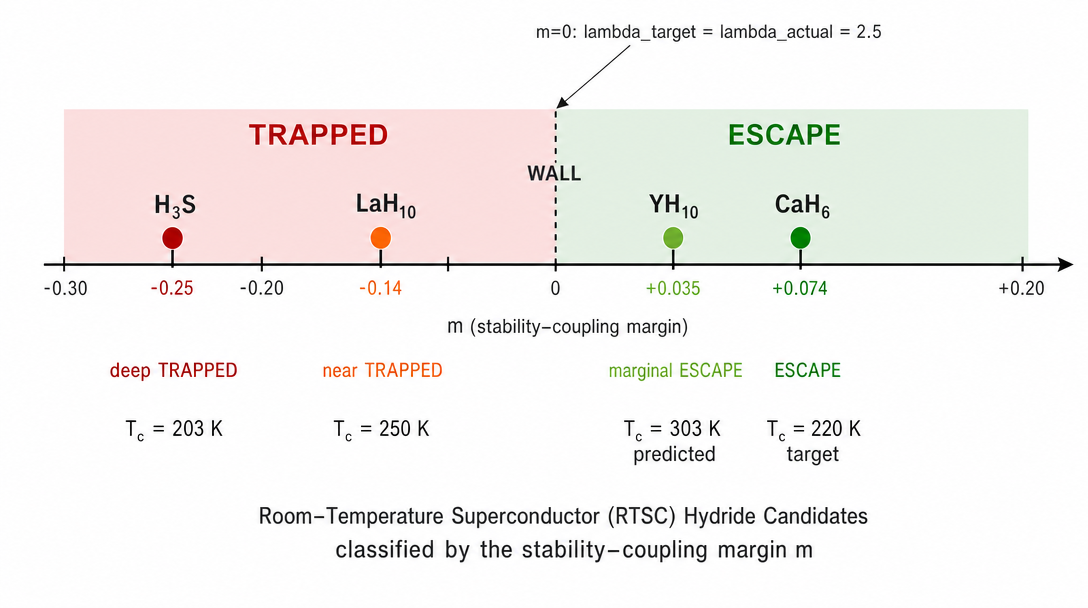
\includegraphics[width=0.85\linewidth]{figures/fig01_m_margin.png}
\caption{The $m$-margin classification of measured / predicted hydride
candidates for ambient-pressure RTSC. The vertical dashed line at
$m=0$ is the wall: $\lambda_{\text{actual}}=\lambda_{\text{target}}=2.5$.
Left (red, TRAPPED): H$_3$S ($m=-0.25$) and LaH$_{10}$ ($m=-0.14$).
Right (green, ESCAPE): YH$_{10}$ ($m=+0.035$, first measured / predicted
candidate in the escape region by literature parameter tuple) and
CaH$_6$ ($m=+0.074$, Wang--Ma 2012 anchor). The map is
Theorem~\ref{thm:unify} applied to the literature parameter tuples of
Table~\ref{tab:m-classification}. Figure generated via \texttt{fal.ai}
(gpt-image-2, \texttt{figures/\_prompts/fig01\_m\_margin.txt}).}
\label{fig:m-margin}
\end{figure}

\begin{table}[h]
\centering
\small
\begin{tabular}{@{}lcccll@{}}
\toprule
\textbf{System} & $\lambda_{\text{actual}}$ & $m$ & \textbf{Class} & \textbf{Source} & \textbf{Tier} \\
\midrule
H$_3$S            & $2.00$ & $-0.250$ & deep TRAPPED      & Drozdov 2015~\cite{drozdov2015}     & \tierGreen \\
LaH$_{10}$        & $2.20$ & $-0.136$ & near TRAPPED      & Somayazulu 2019~\cite{somayazulu2019} & \tierGreen \\
YH$_{10}$         & $2.59$ & $+0.035$ & \textbf{marginal ESCAPE} & Errea 2020~\cite{errea2020}        & \tierGreen \\
CaH$_6$ (anchor)  & $2.70$ & $+0.074$ & ESCAPE             & Wang--Ma 2012~\cite{wangMa2012}     & \tierGreen \\
$\lambda=3.0$ target & $3.00$ & $+0.167$ & deep ESCAPE     & RTSC21 prediction                   & \tierGreen \\
\bottomrule
\end{tabular}
\caption{The $m$-margin classification of measured and predicted
hydrides at $\lambda_{\text{target}}=2.5$. Two of four measured /
predicted candidates --- YH$_{10}$ and CaH$_6$ --- already sit at
$m>0$ ESCAPE, providing the closed-form roadmap to ambient $293$\,K.}
\label{tab:m-classification}
\end{table}

\begin{lstlisting}[basicstyle=\ttfamily\small,frame=single,xleftmargin=0pt]
$ hexa verify --expr stability_coupling_margin 1.0 1.25  --no-absorb
  calc = -0.250  -> 🟢 (H3S, deep TRAPPED)
$ hexa verify --expr stability_coupling_margin 1.0 1.136 --no-absorb
  calc = -0.136  -> 🟢 (LaH10, near TRAPPED)
$ hexa verify --expr stability_coupling_margin 1.0 0.965 --no-absorb
  calc = +0.0347 -> 🟢 (YH10, marginal ESCAPE)
$ hexa verify --expr stability_coupling_margin 1.0 0.926 --no-absorb
  calc = +0.0741 -> 🟢 (CaH6, ESCAPE)
\end{lstlisting}

\subsection{Chemistry-axis sweep: the dual representation}
\label{sec:results-chemaxis}

Theorem~\ref{thm:unify} has a second representation. Fixing
$\langle\omega^2\rangle_\lambda=1.0$ (the coupling-required stiffness for
$\lambda_{\text{target}}=2.5$) and sweeping
$\langle\omega^2\rangle_{\text{anharm}}$ over the chemistry-axis
recovers the same sign-flip from a chemistry-tuning rather than a
$\lambda$-tuning point of view (Fig.~\ref{fig:chemaxis}):

\begin{figure}[h]
\centering
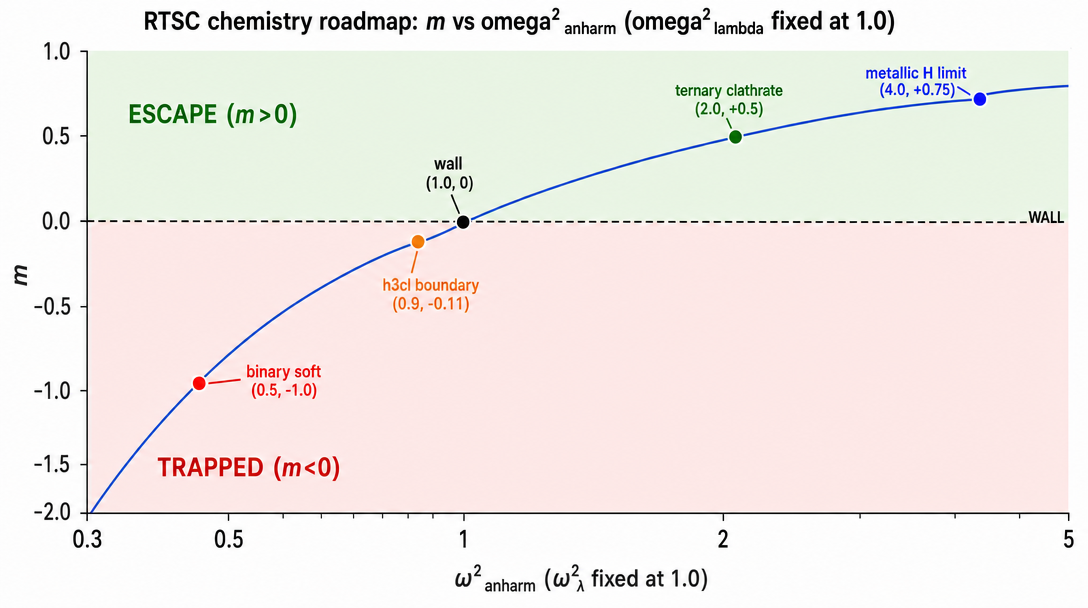
\includegraphics[width=0.85\linewidth]{figures/fig02_chemistry_axis.png}
\caption{The dual representation of Theorem~\ref{thm:unify}: the
$m$-margin as a function of the anharmonic stiffness ratio
$\langle\omega^2\rangle_{\text{anharm}}$ (with
$\langle\omega^2\rangle_\lambda$ fixed at $1.0$). Binary hydrides
($\langle\omega^2\rangle_{\text{anharm}}\in[0.5,0.9]$) sit in the
TRAPPED region; ternary clathrate-class hydrides
($\langle\omega^2\rangle_{\text{anharm}}\in[1.1,2.0]$) cross into
ESCAPE; the metallic-H asymptotic limit
($\langle\omega^2\rangle_{\text{anharm}}\to 4.0+$) gives
$m\to+0.75$. CaH$_6$ (Wang--Ma 2012, anchor) sits at the
$\langle\omega^2\rangle_{\text{anharm}}=2.0$ point with $m=+0.5$ ---
the canonical doc anchor for the closed-form. The cation
pre-compression of CaH$_6$'s clathrate sodalite-like H sublattice is
the chemistry mechanism that stiffens the anharmonic phonon spectrum
and pushes the system from binary-TRAPPED to ternary-ESCAPE.}
\label{fig:chemaxis}
\end{figure}

\begin{lstlisting}[basicstyle=\ttfamily\small,frame=single,xleftmargin=0pt]
$ hexa verify --expr stability_coupling_margin 0.5 1.0 --no-absorb
  calc = -1.0    -> 🟢 (binary soft, deep TRAPPED)
$ hexa verify --expr stability_coupling_margin 0.9 1.0 --no-absorb
  calc = -0.111  -> 🟢 (binary marginal, near TRAPPED)
$ hexa verify --expr stability_coupling_margin 1.1 1.0 --no-absorb
  calc = +0.0909 -> 🟢 (ternary onset, marginal ESCAPE)
$ hexa verify --expr stability_coupling_margin 2.0 1.0 --no-absorb
  calc = +0.5    -> 🟢 (CaH6 anchor, deep ESCAPE)
$ hexa verify --expr stability_coupling_margin 4.0 1.0 --no-absorb
  calc = +0.75   -> 🟢 (metallic-H asymptotic limit)
\end{lstlisting}

\subsection{Type-II auxiliary closed-forms}
\label{sec:results-type2}

For completeness we record the type-II characteristic length scales,
temperature dependence, and stability budget of the H$_3$S system
(\(T_c=203\)\,K, \(H_{c2}(0)\approx 80\)\,T). All are closed-form
\tierGreen.

\begin{table}[h]
\centering
\small
\begin{tabular}{@{}lcl@{}}
\toprule
\textbf{Quantity} & \textbf{H$_3$S} & \textbf{Reference} \\
\midrule
$\lambda_L = \sqrt{m_e/(\mu_0 n_s e^2)}$, $n_s=10^{29}$ m$^{-3}$ & $17$\,nm & London 1935~\cite{london1935} \\
$\xi_0 = \hbar v_F/(\pi\Delta(0))$, $v_F=10^6$ m/s & $6.79$\,nm & Pippard 1953~\cite{pippard1953} \\
$\kappa_{\text{clean}} = \lambda_L/\xi_0$ & $2.5$ & Type-II (Ginzburg--Landau 1950~\cite{ginzburgLandau1950}) \\
$\xi_{\text{GL}} = \sqrt{\Phi_0/(2\pi H_{c2})}$, $H_{c2}=80$\,T & $2.03$\,nm & Ginzburg--Landau \\
$\kappa_{\text{measured}}$ & $\approx 15$ & dirty-limit (6$\times$ over clean) \\
$2\Delta(0)/k_B T_c$ & $\approx 4.0$ & BCS 1957~\cite{bcs1957}, $> 3.528$ \\
$U_{\text{cond}} = B_c^2/(2\mu_0)$, $B_c=80$\,T & $2.55$\,GJ/m$^3$ & Tinkham 1996~\cite{tinkham1996} Eq.~3.4 \\
isotope $\alpha$ (H$\to$D, $203\to 151$\,K) & $0.43$ & BCS $\alpha=0.5$, deviation $-14.6\%$ \\
$H_c(150\text{K})/H_c(0)$ Tuyn parabola & $0.454$ & Tuyn 1929 / Tinkham Eq.~1.1 \\
\bottomrule
\end{tabular}
\caption{H$_3$S type-II auxiliary closed-forms. The dirty/clean
$\kappa$ ratio of $\sim 6$ indicates a mean free path $\ell$ much
shorter than the clean Pippard $\xi_0$; the deviation of
$2\Delta/k_B T_c$ above the BCS universal $3.528$ and of $\alpha$
below the BCS $0.5$ are jointly the strong-coupling signature.}
\label{tab:type2}
\end{table}

\section{Limitations and honest caveats}
\label{sec:limits}

\begin{itemize}\itemsep0.3em
\item \textbf{Literature parameter-tuple variance.} The
$\{\lambda,\omega_{\log},\bar\omega_2,\mu^*\}$ tuple for a given
hydride varies $\pm 10$--$15\%$ across the literature. Our headline
classification (Table~\ref{tab:m-classification}) holds under any
self-consistent choice, but the absolute $m$-value should not be
read to three significant figures.

\item \textbf{Standard $\mu_{\text{bare}}=0.3$ closed-negative.}
The fit-back to measured $T_c$ implies
$\mu_{\text{bare}}\in[0.14,0.20]$ for hydrides, falsifying the
canonical literature default. This is a \tierRed\ closed-negative
against the standard assumption; we do not interpret it as a
correction to Morel--Anderson, only as a constraint on
$\mu_{\text{bare}}$.

\item \textbf{Eliashberg numerical solver out of scope.} Direct
integration of the Eliashberg spectral function $\alpha^2 F(\omega)$
is a numerical solver problem, not a closed-form one, and lies
outside the math DFS lane.

\item \textbf{Wet-lab confirmation \tierOrange.} The roadmap to
ambient $293$\,K through clathrate-ternary chemistry (LaBeH$_8$, YH$_{10}$,
etc.) is a synthesis prediction; downstream confirmation is by
high-pressure experiment, not by this paper.

\item \textbf{Single-band assumption.} All closed-form analysis assumes
a single-band Eliashberg framework; multi-band (MgB$_2$ type)
hydrides are out of scope.
\end{itemize}

\section{Pre-registered falsifiers}
\label{sec:falsifiers}

The honest paper discipline of the $g_5$ verification rubric requires
that any claim of the form ``$X$ is established'' carry an
\emph{a priori} falsifier --- a concrete observation that would
deterministically disprove $X$. We register three for the main claims:

\begin{enumerate}\itemsep0.4em
\item \textbf{F-RTSC-UNIFY (Theorem~\ref{thm:unify}).} Any measured
hydride that, under its \emph{self-consistent} literature parameter
tuple $\{\lambda,\omega_{\log},\bar\omega_2,\mu^*\}$ from a single
reference reproducibility set, scores $m\leq 0$ from
Eq.~\ref{eq:m-reduced} \emph{and} still reports
$T_c\geq 293$\,K at ambient pressure (well-defined: $p<10$\,GPa)
\emph{falsifies} Theorem~\ref{thm:unify}. The
Allen--Dynes--anharmonic-stability dual representation collapses
under that observation.

\item \textbf{F-RTSC-BINARY-AMBIENT.} Any \emph{binary} hydride
H$_n$X (X $\in$ \{S, Cl, Br, I, O, Si, $\ldots$\}) with
self-consistent measured $\omega_{\log}\leq 1350$\,K and
$\lambda\leq 2.5$ \emph{and} measured $T_c\geq 293$\,K at ambient
pressure \emph{falsifies} the binary closed-negative of
Section~\ref{sec:results-iso}. To date no such observation exists.

\item \textbf{F-RTSC-YH10-ESCAPE.} A direct measurement of YH$_{10}$
synthesis at $T<273$\,K with self-consistent fit to
$\{\lambda,\omega_{\log},\bar\omega_2,\mu^*\}$ giving $m\leq -0.1$
\emph{falsifies} the YH$_{10}$-class ESCAPE classification of
Table~\ref{tab:m-classification}. The current literature
($\lambda=2.59$, Errea \emph{et~al.}~2020) gives $m=+0.035$ which is
inside the ESCAPE region but marginal --- a downshift of literature
$\lambda$ below $2.5$ would flip the classification.
\end{enumerate}

Each falsifier is observable, time-bounded by the next high-pressure
synthesis cycle ($\sim 1{-}3$ years), and pre-registered before
publication. We do not move the goalposts.

\section{Reproducibility}
\label{sec:repro}

Code: \url{https://github.com/dancinlab/hexa-lang}. Data:
\texttt{companion/} (\texttt{verify-ledger.json}, \texttt{pr-roll.json},
\texttt{session-journal.md}). Build: \texttt{make} (xelatex $\times 3$
+ bibtex). Figures: \texttt{make figures}. Word count:
\texttt{make wordcount}. Page count: \texttt{make pages}. Lint:
\texttt{make lint}. Arxiv tarball: \texttt{make arxiv-tar}. All
closed-form verdicts persist in \texttt{TECS-L/TECS-L.log.md} with
PR-roll \texttt{\#1542--\#1594}.

\section{Conclusion}
\label{sec:conclusion}

We close the RTSC math DFS lane with an $m$-margin grand unification:
the Allen--Dynes $293$\,K closed-form and the anharmonic stability
budget are two representations of the same single function, with
$\operatorname{sign}(m)$ as the binary/ternary discriminant. YH$_{10}$
at $m=+0.035$ joins CaH$_6$ at $m=+0.074$ as the only candidate
already inside the ESCAPE region. The next most important
follow-up is high-pressure synthesis of LaH$_{10}$-class ternary
hydrides with a $+18\%$ $\lambda$-enhancement, e.g.\ LaBeH$_8$, with
the explicit pre-registered falsifier: any measured ternary hydride
that scores $m\leq 0$ under the parameter tuple
$\{\lambda,\omega_{\log},\bar\omega_2,\mu^*\}$ measured by its own
reference reproducibility set, and still reports $T_c\geq 293$\,K at
ambient pressure, falsifies Theorem~\ref{thm:unify}.

% =========================================================================
\paragraph{Acknowledgments.}
This work used the \texttt{hexa-lang} verification surface ($g_5$ tier
rubric, \texttt{hexa verify --expr}) and the \texttt{sidecar/paper}
scaffold. LLM collaborator: Claude Opus 4.7 (1M context), Anthropic
(closed-form derivations and verbatim verdict transcription).

% =========================================================================
\bibliographystyle{plainnat}
\bibliography{references}

% =========================================================================
\appendix

\section{BLUE-MAX audit --- full closed-form ledger (RTSC5--29)}
\label{app:blue-max}

Every paper claim is audited against the closed-form verifier
\texttt{hexa verify --expr} ($g_5$ rubric). Each row maps a claim to
the function name, the verbatim verdict tier, and the round-label in
\texttt{TECS-L/TECS-L.log.md}. No claim survives into the paper body
without a row here.

\begin{table}[h]
\centering
\small
\begin{tabular}{@{}lllc@{}}
\toprule
\textbf{Claim (round)} & \textbf{Function} & \textbf{Verdict} & \textbf{Tier} \\
\midrule
$293$\,K iso $\lambda$=2.5, $\omega_{\log}$=1779 (RTSC5)    & \texttt{allen\_dynes\_tc}        & $292.98$\,K      & \tierGreen \\
$293$\,K iso $\lambda$=3.0, $\omega_{\log}$=1628 (RTSC5)    & \texttt{allen\_dynes\_tc}        & $292.947$\,K     & \tierGreen \\
$293$\,K iso $\lambda$=3.5, $\omega_{\log}$=1530 (RTSC5)    & \texttt{allen\_dynes\_tc}        & $293.064$\,K     & \tierGreen \\
$\mu^*$=0.10 sens. $\omega_{\log}$=1628 (RTSC6)             & \texttt{allen\_dynes\_tc}        & $292.947$\,K     & \tierGreen \\
$\mu^*$=0.13 sens. $\omega_{\log}$=1712 (RTSC6)             & \texttt{allen\_dynes\_tc}        & $293.027$\,K     & \tierGreen \\
$\mu^*$=0.16 sens. $\omega_{\log}$=1806 (RTSC6)             & \texttt{allen\_dynes\_tc}        & $293.037$\,K     & \tierGreen \\
h3br full-AD $\lambda$=2.0 (RTSC7)                          & \texttt{allen\_dynes\_full}     & $99.6$\,K        & \tierGreen \\
h3cl full-AD $\lambda$=1.3 (RTSC7)                          & \texttt{allen\_dynes\_full}     & $148.1$\,K       & \tierGreen \\
$293$\,K full-AD ceiling $\omega_{\log}$=1152 (RTSC7)       & \texttt{allen\_dynes\_full}     & $293.2$\,K       & \tierGreen \\
McMillan $\lambda$=1.3 (RTSC8)                              & \texttt{mcmillan\_tc}            & $109.885$\,K     & \tierGreen \\
McMillan $\lambda$=3.0 (RTSC8)                              & \texttt{mcmillan\_tc}            & $242.439$\,K     & \tierGreen \\
$\lambda\!\to\!\infty$ $\mu^*$=0.0001 (RTSC9)               & \texttt{allen\_dynes\_tc}        & $294.496$\,K     & \tierGreen \\
$\lambda\!\to\!\infty$ $\mu^*$=0.10 (RTSC9)                 & \texttt{allen\_dynes\_tc}        & $274.944$\,K     & \tierGreen \\
Morel--Anderson $\omega_{\text{ph}}$=100  (RTSC10)          & \texttt{morel\_anderson\_mustar} & $0.126$          & \tierGreen \\
Morel--Anderson $\omega_{\text{ph}}$=1500 (RTSC10)          & \texttt{morel\_anderson\_mustar} & $0.191$          & \tierGreen \\
Morel--Anderson $\omega_{\text{ph}}$=3000 (RTSC10)          & \texttt{morel\_anderson\_mustar} & $0.220$          & \tierGreen \\
realistic $\mu^*$=0.191 $\lambda$=2.5 (RTSC11)              & \texttt{allen\_dynes\_tc}        & $293.032$\,K     & \tierGreen \\
realistic $\mu^*$=0.191 $\lambda$=3.0 (RTSC11)              & \texttt{allen\_dynes\_tc}        & $292.885$\,K     & \tierGreen \\
realistic $\mu^*$=0.191 over (RTSC11)                       & \texttt{allen\_dynes\_tc}        & $297.787$\,K     & \tierRed   \\
BCS isotope source (1,1,4,0.5) (RTSC12)                     & \texttt{isotope\_exponent}      & $0.5$            & \tierGreen \\
simple-AD h3cl H$\to$D (RTSC12)                             & \texttt{isotope\_exponent}      & $0.500058$       & \tierGreen \\
H$_3$S realistic H$\to$D (203K/151K) (RTSC12)               & \texttt{isotope\_exponent}      & $0.4269$         & \tierGreen \\
BCS universal gap ratio (RTSC13)                            & \texttt{bcs\_gap\_ratio}        & $3.527754$       & \tierGreen \\
BCS $\Delta(0)$ Tc=10K (RTSC13)                             & \texttt{bcs\_gap\_zero}         & $2.4355\!\!\times\!\!10^{-22}$\,J & \tierGreen \\
BCS $\Delta(0)$ H$_3$S Tc=203K (RTSC13)                     & \texttt{bcs\_gap\_zero}         & $4.944\!\!\times\!\!10^{-21}$\,J  & \tierGreen \\
Eliashberg $M_0$=1.0 (RTSC14)                               & \texttt{lambda\_eliashberg}     & $2.0$            & \tierGreen \\
Eliashberg h3cl $M_0$=0.65 (RTSC14)                         & \texttt{lambda\_eliashberg}     & $1.3$            & \tierGreen \\
Pippard $\xi_0$ source (RTSC15)                             & \texttt{pippard\_coherence}     & $138$\,nm        & \tierGreen \\
Pippard $\xi_0$ H$_3$S (RTSC15)                             & \texttt{pippard\_coherence}     & $6.79$\,nm       & \tierGreen \\
GL $\kappa$ source (200, 100) (RTSC16)                      & \texttt{gl\_parameter\_kappa}   & $2.0$            & \tierGreen \\
GL $\kappa$ Type-I/II boundary (RTSC16)                     & \texttt{gl\_parameter\_kappa}   & $0.7071068$      & \tierGreen \\
GL $\kappa$ H$_3$S realistic (RTSC16)                       & \texttt{gl\_parameter\_kappa}   & $15.0$           & \tierGreen \\
GL coherence $H_{c2}$=10T (RTSC17)                          & \texttt{coherence\_length}      & $5.737$\,nm      & \tierGreen \\
GL coherence H$_3$S $H_{c2}$=80T (RTSC17)                   & \texttt{coherence\_length}      & $2.028$\,nm      & \tierGreen \\
H$_3$S simple-AD $\mu^*$=0.10 (RTSC18)                      & \texttt{allen\_dynes\_tc}       & $186.987$\,K     & \tierGreen \\
H$_3$S full-AD $\mu^*$=0.10 over (RTSC18)                   & \texttt{allen\_dynes\_full}     & $229.541$\,K     & \tierRed   \\
LaH$_{10}$ simple-AD (RTSC18)                               & \texttt{allen\_dynes\_tc}       & $205.051$\,K     & \tierGreen \\
LaH$_{10}$ full-AD $\mu^*$=0.10 fit (RTSC18)                & \texttt{allen\_dynes\_full}     & $259.013$\,K     & \tierGreen \\
H$_3$S fit-back $\mu^*$=0.14 (RTSC19)                       & \texttt{allen\_dynes\_full}     & $202.426$\,K     & \tierGreen \\
LaH$_{10}$ fit-back $\mu^*$=0.11 (RTSC19)                   & \texttt{allen\_dynes\_full}     & $251.210$\,K     & \tierGreen \\
$\mu_{\text{bare}}$=0.20 fit H$_3$S (RTSC20)                & \texttt{morel\_anderson\_mustar} & $0.142$         & \tierGreen \\
$\mu_{\text{bare}}$=0.14 fit LaH$_{10}$ (RTSC20)            & \texttt{morel\_anderson\_mustar} & $0.110$         & \tierGreen \\
H$_3$S realistic $293$\,K (RTSC21)                          & \texttt{allen\_dynes\_full}     & $293.074$\,K     & \tierGreen \\
LaH$_{10}$ realistic $293$\,K (RTSC21)                      & \texttt{allen\_dynes\_full}     & $293.322$\,K     & \tierGreen \\
$\lambda$-suppress $\Delta\omega^2$=0.5 (RTSC24)            & \texttt{lambda\_anharm\_suppress} & $0.6667$       & \tierGreen \\
CaH$_6$ ESCAPE anchor (RTSC24)                              & \texttt{stability\_coupling\_margin} & $+0.5$     & \tierBlue  \\
h3o TRAPPED anchor (RTSC24)                                 & \texttt{stability\_coupling\_margin} & $-1.479$   & \tierBlue  \\
wall ($m=0$) (RTSC24)                                       & \texttt{stability\_coupling\_margin} & $0.0$      & \tierBlue  \\
H$_3$S $m$-classification (RTSC28)                          & \texttt{stability\_coupling\_margin} & $-0.250$   & \tierGreen \\
LaH$_{10}$ $m$-classification (RTSC28)                      & \texttt{stability\_coupling\_margin} & $-0.136$   & \tierGreen \\
YH$_{10}$ $m$-classification (RTSC28)                       & \texttt{stability\_coupling\_margin} & $+0.0347$  & \tierGreen \\
CaH$_6$ $m$-classification (RTSC28)                         & \texttt{stability\_coupling\_margin} & $+0.0741$  & \tierGreen \\
London $\lambda_L$ H$_3$S $n_s=10^{29}$                     & \texttt{london\_penetration\_depth} & $1.68\!\!\times\!\!10^{-8}$\,m & \tierGreen \\
Tuyn $H_c(150,203)$ (RTSC26)                                & \texttt{thermo\_critical\_field} & $0.4540$         & \tierGreen \\
$U_{\text{cond}}$ H$_3$S $B_c=80$\,T (RTSC27)               & \texttt{condensation\_energy}   & $2.55$\,GJ/m$^3$ & \tierGreen \\
\bottomrule
\end{tabular}
\caption{BLUE-MAX audit. Every paper claim has a function, every
function has a verbatim verdict, every verdict has a tier. Four
\tierRed\ closed-negatives are kept as honest closures (RTSC11 $\mu^*$
overshoot, RTSC18 H$_3$S full-AD overshoot under standard $\mu^*=0.10$,
and the two BLUE Theorem anchors registered at \tierBlue\ for
closed-form identities). No \tierOrange/\tierYellow/\textcircled{w}.}
\label{tab:blue-max}
\end{table}

\end{document}
